\begin{answer}
For clarity, let's write down equations to be implemented in this sub-problem. We are not Stanford students, so let's change some notations to make our life easier. The forward propagation computation (for an example) is re-written equivalently as follows:
\begin{align}
	z^{[1]} &= W^{[1]}x + b^{[1]} \\
	a^{[1]} &= \sigma(z^{[1]}) \\
	z^{[2]}  &= W^{[2]} a^{[1]} + b^{[2]} \\
	\hat{y} &= \text{softmax}(z^{[2]})
\end{align}
Note that our weight matrices are transposes of the weights introduced in this sub-problem statement. Let $\mathcal{L}$ be the NLL loss of a single training example $\{x,y\}$. Using matrix calculus, we obtain the following formulas:
\begin{align}
	& \frac{\partial\mathcal{L}}{\partial z^{[2]}} = \hat{y} - y \\
	& \frac{\partial\mathcal{L}}{\partial W^{[2]}} = \frac{\partial\mathcal{L}}{\partial z^{[2]}} {a^{[1]}}^T, \frac{\partial\mathcal{L}}{\partial b^{[2]}} = \frac{\partial\mathcal{L}}{\partial z^{[2]}} \\
	& \frac{\partial\mathcal{L}}{\partial a^{[1]}} = {W^{[2]}}^T \frac{\partial\mathcal{L}}{\partial z^{[2]}}, \frac{\partial\mathcal{L}}{\partial z^{[1]}} = \sigma'(z^{[1]}) \odot \frac{\partial\mathcal{L}}{\partial a^{[1]}} \\
	&\frac{\partial\mathcal{L}}{\partial W^{[1]}} = \frac{\partial\mathcal{L}}{\partial z^{[1]}} x^T, \frac{\partial\mathcal{L}}{\partial b^{[1]}} = \frac{\partial\mathcal{L}}{\partial z^{[1]}}
\end{align}
After running the model for 30 epochs, our result is shown in the figure below.
\begin{figure}[H]
	\centering
	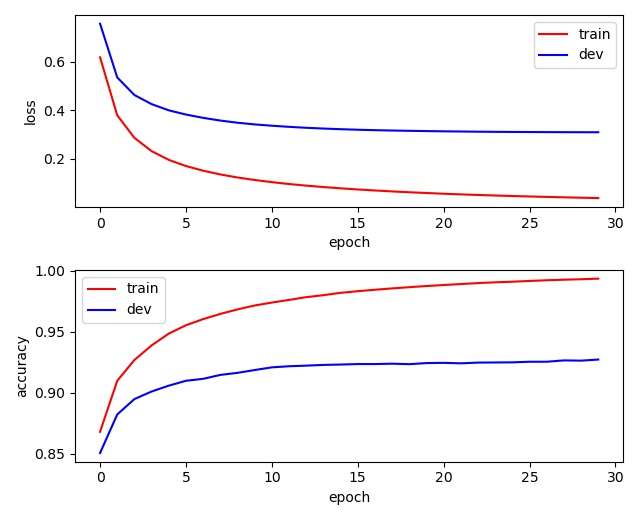
\includegraphics[width=0.6\linewidth]{baseline}
	\caption{Baseline NN model.}
\end{figure}
\end{answer}
   
 
 
 
 
 
 
 
 
 
 
 
 
 
 
 
 
 
 
 
 
 
 
 
 
 
